\section{Spike-Driven Dreamer}
\label{sec:method}

\begin{figure*}[t]
  \centering
  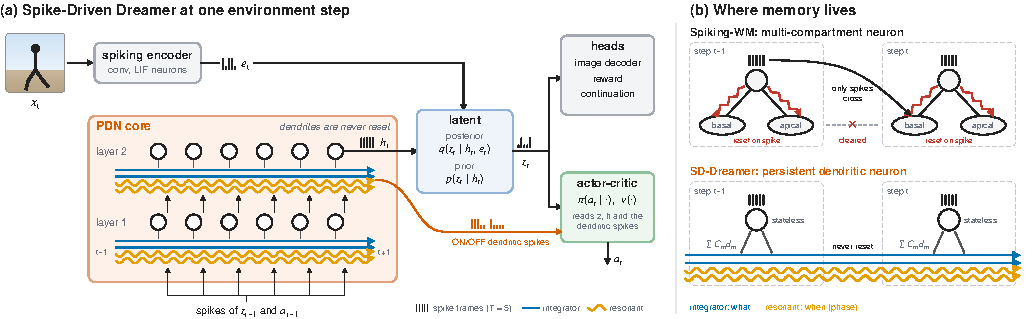
\includegraphics[width=\textwidth]{fig/overview}
  \caption{\textbf{\methodfull.}
  (a) Two layers of persistent dendritic neurons (PDNs) form the recurrent core of a spiking Dreamer. Each neuron has an integrator (blue) and a resonant (orange) dendritic channel; PDM carries them across environment steps without reset, and NWG writes into them on one scale for every retention time. Its stateless soma sends a spike count over the $T=5$ simulation steps, and the spikes of a layer also feed back into its dendrites ($R$). The actor and critic also read the dendrites of the second layer as ON and OFF spikes.
  (b) In \swm, all compartments are cleared at every step and the dendrites at every somatic spike, so only spikes reach the next step. In a PDN, PDM keeps the dendritic channels across steps; spikes add to them but never clear them.}
  \label{fig:overview}
\end{figure*}

\method follows the design rule of \cref{sec:amnesia}: it keeps the spiking world model of \cref{sec:swm} and replaces its MCN sequence model with two layers of persistent dendritic neurons (PDNs), as shown in \cref{fig:overview}.
The encoder, the dynamics predictor, the heads and the actor-critic remain LIF networks trained with the losses of DreamerV3~\cite{hafner2025dreamerv3}.
A PDN separates memory from communication and consists of three parts: (i) Persistent Dendritic Memory (PDM), which keeps the state of its dendritic channels across environment steps and somatic spikes (\cref{sec:pdm}); (ii) the Normalized Write Gain (NWG), which writes the synaptic current into channels of every retention time on one scale (\cref{sec:nwg}); and (iii) a stateless soma, which reads the channels and emits spikes (\cref{sec:soma}).

A PDN layer has $N$ neurons with $M$ dendritic channels each and is updated once per environment step.
At step $t$, it receives the firing rate $x_t$ of its input spikes over the $T$ simulation steps and its own firing rate $\bar s_{t-1}$ of the previous step, and computes
\begin{equation}
\begin{aligned}
I_t &= \LN\big(B x_t + R\,\bar s_{t-1}\big),\\
d_t &= \mathrm{PDM}\big(d_{t-1}, I_t\big), \quad s_t = \mathrm{Soma}\big(d_t, x_t\big).
\end{aligned}
\label{eq:input}
\end{equation}
Here, $B$ and $R$ are synaptic matrices, $\LN$ is layer normalization~\cite{ba2016layernorm}, $I_t\in\mathbb{R}^{NM}$ is the synaptic current into the dendrites, $d_t\in\mathbb{C}^{NM}$ is the dendritic state, and $s_t\in\{0,1\}^{T\times N}$ are the spikes of the layer over the $T$ simulation steps.
The first layer reads the input spikes of the sequence model, which encode $(z_{t-1},a_{t-1})$, the second layer reads the spikes of the first, and the spikes of the second layer form the deterministic state $h_t$.

\subsection{Persistent Dendritic Memory}
\label{sec:pdm}

\Cref{sec:amnesia} shows that the step reset and the spike reset confine the memory of a spiking neuron to at most one environment step.
A memory that spans many steps therefore needs a dendritic state that neither reset touches.
To this end, PDM updates each dendritic channel once per environment step with the discretized dynamics of a resonate-and-fire neuron~\cite{izhikevich2001resonate}, a damped rotation driven by the current:
\begin{equation}
d_t = \lambda\, e^{i\theta}\, d_{t-1} + g(\lambda)\, I_t, \qquad \lambda = e^{-1/\tau}.
\label{eq:pdm}
\end{equation}
Here, all operations are elementwise; each channel has a retention time $\tau$, counted in environment steps, and a phase $\theta$, both learned, and $g(\lambda)$ is the write gain of \cref{sec:nwg}.
A channel with $\theta=0$ is an integrator, whose state stays real and follows the leaky trace $d_t=\lambda d_{t-1}+g(\lambda)I_t$; a channel with $\theta\neq0$ is a resonator, a damped oscillator.

\Cref{eq:pdm} is the only update of the channels.
Their state is carried across environment steps, through training sequences and imagination rollouts, and is cleared only at the start of an episode; the spikes of the layer reach it only as current through $R$, so no spike resets it.
The contribution of a current $k$ steps back, $g(\lambda)\lambda^{k}e^{ik\theta}I_{t-k}$, is therefore independent of the spikes the neuron emitted in between, and its gradient crosses no surrogate derivative.
The two kinds of channels store complementary information.
An integrator stores what was observed, superposing inputs of all ages with the weights $\lambda^{k}$.
A resonator also stores when: an input of age $k$ carries the phase $k\theta$, which separates it from inputs of age $k\pm1$.

\subsection{Normalized Write Gain}
\label{sec:nwg}

PDM keeps a trace for about $\tau$ environment steps, but a long retention time is useful only if the trace is strong enough to drive the soma.
With the Euler gain of \cref{eq:lif,eq:mcn}, $g(\lambda)=1-\lambda\approx1/\tau$, a current of unit variance gives a state of variance about $1/(2\tau)$ (\cref{sec:amnesia}), so the channels with the longest retention times store their input most faintly.
NWG instead sets the write gain to the normalization of the LRU~\cite{orvieto2023lru}:
\begin{equation}
g(\lambda)=\sqrt{1-\lambda^2}.
\label{eq:nwg}
\end{equation}
For a current of unit variance that is uncorrelated over time, the stationary variance of every channel becomes $(1-\lambda^2)\sum_{k\ge0}\lambda^{2k}=1$, independent of $\tau$.
All channels thus write on one scale, and one layer can hold a wide spectrum of retention times: we initialize $\tau$ log-uniformly in $[1,1000]$ environment steps and learn it, so no time constant is tuned for a task.

\subsection{Stateless soma and policy input}
\label{sec:soma}

The soma passes the dendritic memory to the next layer, the feedback $R$ and the rest of the world model as spikes.
Since PDM holds the memory, the soma needs no state of its own: at every environment step it reads the channels of its neuron and the direct input, and emits a spike count over the $T$ simulation steps,
\begin{equation}
\begin{aligned}
u_t &= \textstyle\sum_{m=1}^{M} \mathrm{Re}\big(c_m \odot d_{t,m}\big) + D x_t,\\
s_t[n] &= \Hv\big(\LN(u_t) - n\vartheta/T\big), \quad n=1,\dots,T.
\end{aligned}
\label{eq:soma}
\end{equation}
Here, $d_{t,m}\in\mathbb{C}^{N}$ is the $m$-th channel of every neuron, $c_m\in\mathbb{C}^{N}$ are readout weights, $D$ is a synaptic matrix and $\vartheta=0.5$ is the threshold.
The spike count encodes $\LN(u_t)$ in $T+1$ levels, whereas one spike per environment step carries a single bit.
The soma keeps no state between environment steps, so no reset touches the memory, and its binary spikes are the only signal the neuron sends; the next layer and the feedback read their rate $\bar s_t$.
The synaptic operations $Bx_t$, $R\bar s_{t-1}$ and $Dx_t$ therefore act on spikes, and the dendritic update is local to each neuron, with $O(NM)$ operations per step against $O(N^2)$ for the recurrent matrix of a GRU.
The Heaviside steps are trained with the surrogate derivative of \swm.

The actor and critic read $z_t$, $h_t$ and the dendritic state of the second layer, which holds the memory directly; the Memory Maze probes read the same features.
To keep their input binary, the real part of every channel and the imaginary part of every resonator, each standardized over the layer, are compared with $T$ positive and $T$ negative thresholds $\pm(n-\tfrac12)\tfrac{2}{T}$, $n=1,\dots,T$, which yields $2T$ ON and OFF spike frames per environment step.
Supp.~\suppref{supp:policy}{E} compares a policy that reads $(z_t,h_t)$ only.
